\documentclass{beamer}
\usepackage{preamble}

\title{Coding for Humanities}
\author{Andreas van Cranenburgh}
\date{Week 6: Tabular data analysis with Pandas}

\begin{document}
\maketitle




\begin{frame}{Program for today}
\tableofcontents
\end{frame}


\section{Midterm feedback}

\begin{frame}{Midterm feedback}
    \begin{itemize}
        \item Most of your code was pretty good!
        \item We'll review some things to pay attention to.
    \end{itemize}
\end{frame}

\begin{frame}{Always report requested results!}
    Read the questions carefully. \\
    When results are requested, include them!
    \begin{itemize}
        \item Suppose that we call function \textcolor{blue}{\texttt{a}}
            as follows: [...]\\
            What values will be printed to the screen?
        \item Use [your function] to print all tweets addressed to @FLOTUS.
        \item Count the \#hashtags and \@usernames in Trump's tweets, and
            report the top 10 for both.
    \end{itemize}
\end{frame}


\begin{frame}[fragile]{Functions: return vs print}
Write a function first\_letters(filename) that reads a poem in a text file
\structure{and returns a string of first letters} of all of its lines.
\vspace{1em}
\begin{columns}
\column{0.5\textwidth}
Don't print inside the function:
\begin{lstlisting}[style=smaller]
def first_letters(text):
    punctuation = '...'
    for char in punctuation:
        text = text.replace(char, '')
    for line in text.splitlines():
        print(line[0])
\end{lstlisting}
\pause\column{0.5\textwidth}
Collect and \structure{return} the result: 
\begin{lstlisting}[style=smaller]
def first_letters(text):
    punctuation = '...'
    for char in punctuation:
        text = text.replace(char, '')
    result = ''
    for line in text.splitlines():
        result += line[0]
    return result
\end{lstlisting}
\end{columns}
\end{frame}

\begin{frame}[fragile]{Functions: making re-usable functions}
\begin{lstlisting}[style=smaller]
prefix = '@'

def filter_ats(tokens, prefix):
    newlist = [k for k in tokens if prefix in k]
    return newlist

usernames = filter_ats(tokens, prefix)

prefix2 = '#'

def filter_hashtags(tokens, prefix2):
    newlist = [k for k in tokens if prefix2 in k]
    return newlist

hashtags = filter_hashtags(tokens, prefix2)
\end{lstlisting}

(BTW: great use of list comprehensions)
\end{frame}

\begin{frame}[fragile]{Functions: making re-usable functions}
One re-usable function: 
\begin{lstlisting}[style=smaller]
def filter_tokens(tokens, prefix):
    newlist = [token for token in tokens
            if token[0] == prefix]
    return newlist

usernames = filter_tokens(tokens, '@')
hashtags = filter_tokens(tokens, '#')
\end{lstlisting}

Lesson:
    \begin{itemize}
        \item Don't Repeat Yourself (DRY)
        \item one function can do multiple jobs,
            based on its arguments
    \end{itemize}
\end{frame}

\begin{frame}[fragile]{Function scope}
    \begin{definition}
        The \structure{scope} of a variable determines
            which parts of your code can access a variable.
    \end{definition}
    \begin{description}
        \item[global scope]
            variables created outside a function.
            Everyone can see them!
        \item[local scope]
            arguments of and variables created in a function.
            Other code cannot see it!
    \end{description}
\end{frame}


\begin{frame}[fragile]{What if there are more than 2 punctuation marks?}
    \begin{columns}[T]
\column{0.6\textwidth}
Skipping only the first punctuation mark is not enough!
\begin{lstlisting}[style=plain]
- ``Shall I compare thee ...''
- ``Please don't!'' she replied
\end{lstlisting} % SPAM
\pause\column{0.4\textwidth}
Solution: remove all punctuation
\begin{lstlisting}[style=plain]
Shall I compare thee
Please dont
\end{lstlisting}
\end{columns}
Lesson:
    \begin{itemize}
        \item Don't just test your code \\
            on the particular given examples.
        \item Tests are typically not exhaustive
        \item Reflect whether you really solved the problem.
    \end{itemize}
\end{frame}

\begin{frame}[fragile]{For loops: premature return}
\begin{columns}
\column{0.5\textwidth}
Pay attention to what is part of a for loop!
\begin{lstlisting}
result = []
for line in text.splitlines():
    result += line[0]
    return result
\end{lstlisting}
Why does this not work?
\texttt{return} immediately aborts the function!
\pause\column{0.5\textwidth}
\begin{lstlisting}
result = []
for line in text.splitlines():
    result += line[0]
return result
\end{lstlisting}
\end{columns}
\end{frame}

\begin{frame}[fragile]{For loops: inefficiency}
\begin{columns}
\column{0.5\textwidth}
Pay attention to what is part of a for loop!
\begin{lstlisting}
chars = []
for line in text.splitlines():
    chars.append(line[0])
    result = ''.join(chars)
return result
\end{lstlisting}
This repeats the join at every iteration, completely unnecessary!
\pause\column{0.5\textwidth}
Solution: Take the join out of the for loop:
\begin{lstlisting}
chars = []
for line in text.splitlines():
    chars.append(line[0])
result = ''.join(chars)
return result
\end{lstlisting}
\end{columns}
\end{frame}

\begin{frame}[fragile]{Only concatenate same types!}
\begin{columns}[T]
\column{0.5\textwidth}
Don't do this:
\begin{lstlisting}
result = []
for line in text.splitlines():
    result += line[0]
\end{lstlisting}
Why not? Type mismatch:
    \begin{itemize}
        \item \texttt{result} is a list
        \item \texttt{line[0]} is a string \\
            (of one character).
    \end{itemize}
\pause\column{0.5\textwidth}
Better:
\begin{lstlisting}
result = ''
for line in text.splitlines():
    result += line[0]
\end{lstlisting}
Best:
\begin{lstlisting}
return ''.join(line[0] for line
        in text.splitlines())
\end{lstlisting}
\end{columns}
\end{frame}


\begin{frame}{Summary}
    Most of your code was pretty good!
    
    \vspace{1em}
    Pay attention to:
    \begin{itemize}
        \item functions
        \item indendation
        \item types
    \end{itemize}
\end{frame}





\section{Exploratory Data Analysis}
\frame{\tableofcontents[currentsection]}

\begin{frame}{Definition}
    \begin{definition}
    \structure{Data science} is the application of
    computational and statistical techniques to
    address or gain [managerial or scientific]
    insight into some problem in the real world.
    --- Zico Kolter, Machine Learning Prof, CMU
    \end{definition}
\end{frame}


\begin{frame}
    \centering
    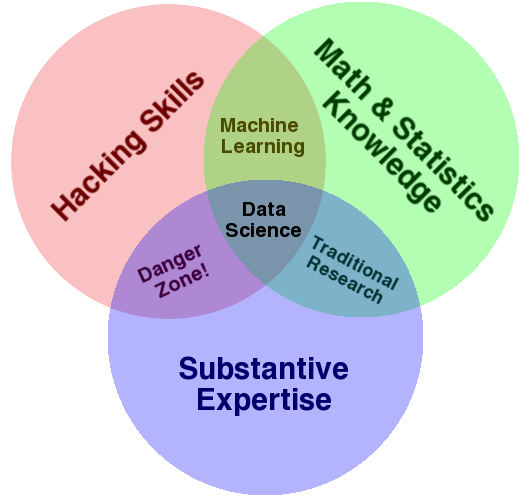
\includegraphics[height=0.8\textheight]{fig/venn}

    Drew Conway

    CEO, Alluvium (analytics company)
\end{frame}


\begin{frame}{The Data Lifecycle}
    \begin{enumerate}
        \item Data collection
        \item Data processing
        \item \structure{Exploratory analysis \& visualization}
        \item Analysis, hypothesis testing, \& Machine Learning
        \item Insight \& Policy Decision
    \end{enumerate}

    Today: focus on step 3
\end{frame}

\begin{frame}{Data Collection, Processing}
In practice, this often takes the most time (up to 80\%!)

\begin{itemize}
    \item Acquiring data
        \begin{itemize}
            \item Scrape from web, PDFs
            \item Database dump
            \item etc.
        \end{itemize}
    \item Messy data: encoding issues, date formats, order of first/last names, etc.
    \item Missing data
    \item Converting data
        \begin{description}
            \item[Tidy format] one observation per row, \\
                    each variable is a column
        \end{description}
\end{itemize}
\end{frame}



\begin{frame}{Types of variables}
    \begin{description}
        \item[Continuous] numerical variables\\
            age, length, etc.
        \item[Categorical] predefined set of values\\
            yes/no, True/False, red/blue/green, etc.
        \item[Text] open-ended \\
            comments, tweets, etc.
    \end{description}
\end{frame}

\begin{frame}{Descriptive statistics}
%Part of \structure{descriptive statistics}, used to summarize data:
%\begin{itemize}
%    \item Convey lots of information with extreme simplicity
%\end{itemize}

Descriptive statistics for one variable:
\begin{itemize}
    \item Distribution: bar plot, histogram
    \item Measures of location: mean, median
    \item Measure of dispersion: standard deviation
\end{itemize}

Measuring correlation of two variables:
\begin{itemize}
    \item Scatter plots
    \item Understanding correlation
    \item Measuring correlation
\end{itemize}
\end{frame}

\subsection{Exploring one variable}

\begin{frame}{Plotting a distribution: categorical}
Collected favorite color of 100 people:

[black, green, green, blue, red, \dots ]

\vspace{1em}
How do we visualize this?

\pause
A bar plot:

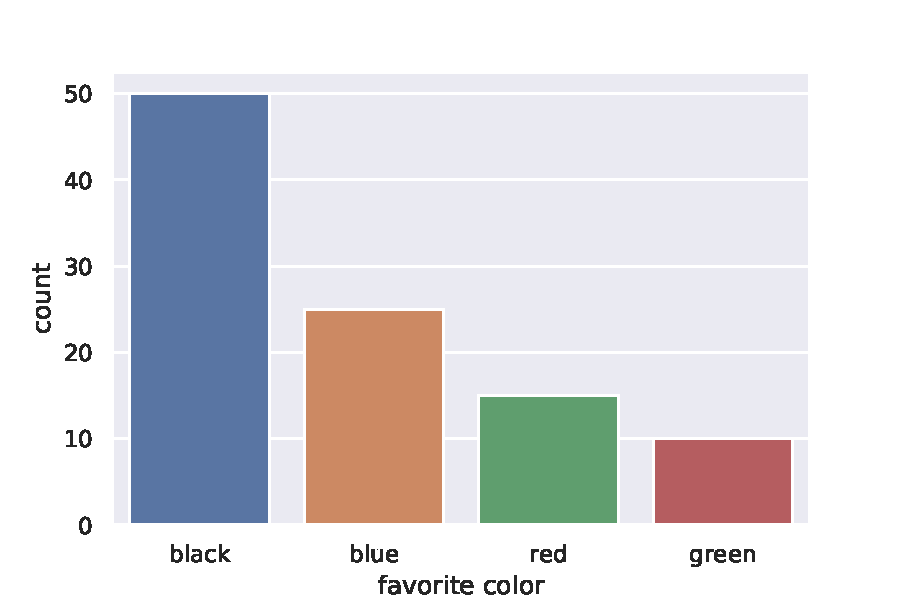
\includegraphics[width=0.7\textwidth]{fig/barplot}

Don't use a pie chart: \url{https://www.businessinsider.com/pie-charts-are-the-worst-2013-6}
\end{frame}


\begin{frame}{Plotting a distribution: continuous}
Collected height of 100 people:

[1.85, 1.66, 1.77, 1.68, \dots]

\vspace{1em}
How do we visualize this?

\pause
A histogram:

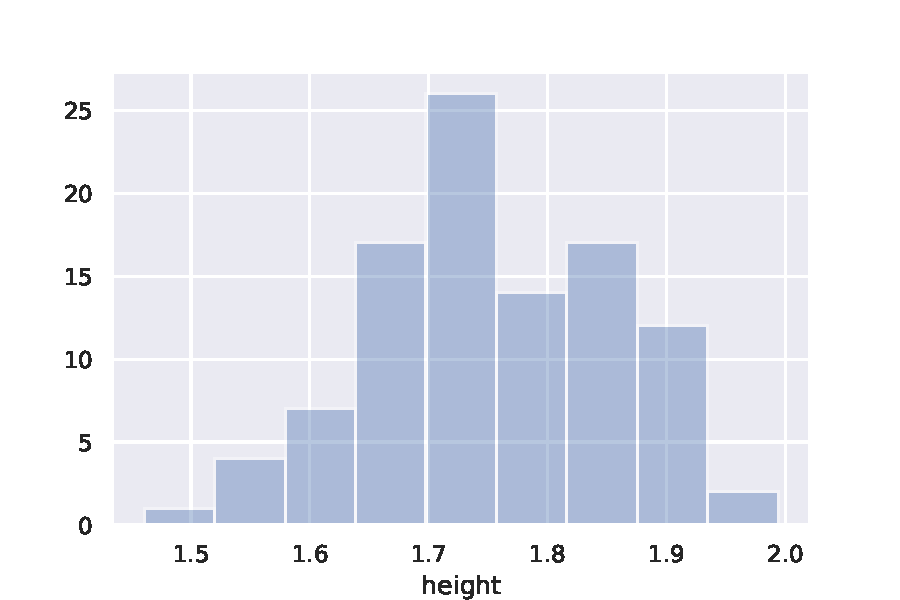
\includegraphics[width=0.8\textwidth]{fig/histogram}
\end{frame}



\begin{frame}{Average house price in each US state}
\begin{columns}
\column{0.5\textwidth}
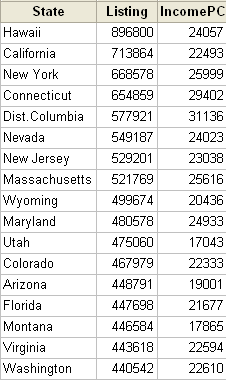
\includegraphics[height=0.8\textheight]{fig/housepricesincome}
\column{0.5\textwidth}
What is the average price across the whole US?

\pause\vspace{1em}
price = (hawaii + california \\
    + ... ) / 50 = \$ 369,687

\vspace{1em}
Is this a fair summary?
\end{columns}
\end{frame}

\begin{frame}{Averaging averages?}
\structure{But}:

Hawaii's average listing = \$896,800\\
Hawaii's population = 1,275,194\\
Illinois' average listing = \$377,683\\
Illinois' population = 12,763,371

\vspace{1em}
Each state gets a weight of 1/50.\\
Hawaii would have too much influence.

\pause
\structure{Better}:
\begin{block}{Weighted average}
price = (weight$_1 \times $value$_1$ + weight$_2 \times $value$_2$ + \dots)

    where weight is population$_{\textsf{state}}$ / population$_{\textsf{total}}$
\end{block}

\vspace{1em}
New average is \$409,234 compared to \$369,687 without weights,
an error of 11\%
\end{frame}


\begin{frame}{Mean and median}
`Average' can mean different things:
\begin{description}
\item[Mean] sum of values, divided by number of values \\
        Mean[1,2,4,6,8,9,17] = 47 / 7 = 6.71\dots

\item[Median] sort data, take the middle point

    \begin{description}
    \item[Odd length:]
        Med[1,2,4,\structure{6},8,9,17] = 6

    \item[Even length:]
        Midpoint between the two central observations \\
        Med[1,2,4,\structure{6,8},9,14,17] = (6+8)/2 = 7
    \end{description}
    %\item[Mode] most common value
    %\item[Harmonic/geometric mean]
\end{description}
\end{frame}

\begin{frame}{Skewness}
Extreme observations distort means but not medians:
\begin{itemize}
\item Med [1,2,4,6,8,9,17] = 6
\item Mean[1,2,4,6,8,9,17] = 6.714
\item Med [1,2,4,6,8,9,17000] = 6 (still)
\item Mean[1,2,4,6,8,9,17000] = 2432.8 (!)
\end{itemize}
Typically occurs when there are outliers,
such as in cross sections of income or wealth
and/or when the sample is not very large.
\end{frame}

\begin{frame}{Measuring dispersion: use range min/max?}
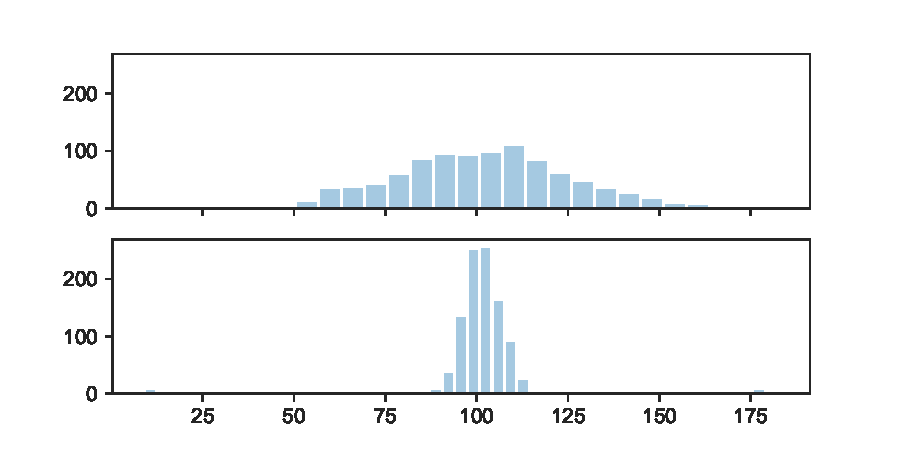
\includegraphics[width=0.9\textwidth]{fig/disp}

These two datasets both have 1,000 observations \\
that range from about 10 to about 180.
\end{frame}


\begin{frame}{Standard deviation}
A measure of the amount of variation,\\
in the same unit as the original data

\begin{description}
    \item[Low SD:] values tend to be close to the mean
    \item[High SD:] values can be much lower and/or higher than the mean
\end{description}

\begin{block}{Example}
normal distribution with mean 10 and SD 3, then:\\
68\% of values are within 1 SD of mean (between 7 and 13) \\
95\% of values are within 2 SDs of mean (between 4 and 16) \\
99.7\% \dots
\dots
\end{block}
\end{frame}

\begin{frame}{Summary: inspecting one variable}
\begin{tabular}{lll}     & categorical & continuous \\
1. Plot its distribution & bar plot    & histogram \\
2. Central tendency      & -           & mean, median \\
3. Dispersion            & -           & range, standard deviation \\
\end{tabular}
\end{frame}




\section{Reproducible research with Pandas}
\frame{\tableofcontents[currentsection]}

\begin{frame}{Intermezzo: reproducibility}
    \structure{Austerity policy}.

    Time line:
    \begin{itemize}
        \item 2008: Economic recession/crisis
        \item Reinhart \& Rogoff (2010) analyze correlation between debt and economic growth \\
            \begin{block}{Claim:}
            debt should be less than 90\% of GDP, otherwise economic growth drops dramatically
            \end{block}
        \item Austerity policy in EU, Greece needs to reduce debt etc.
    \end{itemize}
\end{frame}

\begin{frame}{The dangers of Excel}
    Problem:
    \begin{itemize}
        \item The claim is wrong. They made a crucial mistake in their Excel sheet!
        \item Excel hides formulas, easy to overlook mistakes
        \item Can we do better with Python?
    \end{itemize}

    \vspace{1em}
    \url{https://www.nytimes.com/2013/04/19/opinion/krugman-the-excel-depression.html}
\end{frame}

\begin{frame}{Reproducibility}
    Research should be reproducible:

    \begin{itemize}
        \item Code and data should be made available (if possible)
        \item Version control for code and data
        \item Ensure code still works 20+ years later. \\
                Hard problem: bit rot.
        \item Check code/data in peer review \\
            However, this requires lots of time and expertise; realistic?
    \end{itemize}

    Some overlap between open source, open science, open data, open access, etc.
\end{frame}

% Plug notebooks again




\subsection{Analyzing results with Pandas}
\begin{frame}{Pandas}
    Pandas: versatile data analysis tool \dots

    \begin{itemize}
        \item Load/write tabular data (csv, excel)
        \item Manipulate/process data
        \item Analyze: e.g., basic statistics
        \item Plot: look at data, interactions, etc.
    \end{itemize}
\end{frame}

\begin{frame}{The main datastructures}
    \begin{description}
        \item[Series:] one-dimensional, indexed array of numbers or strings
            \begin{itemize}
                \item ordered (like list)
                \item indexed: lookup items by key (like dict)
                \item mutable
            \end{itemize}
        \item[DataFrame:] two-dimensional table with Series as columns.
            \begin{itemize}
                \item Rows are instances (observations, individuals, etc.)
                \item Columns are features (e.g., age, length, etc.)
            \end{itemize}
            %Each column is a series with a single type (homogeneous), \\
            %but a data frame can contain columns of different types (heterogeneous).
    \end{description}
\end{frame}

% don't show the mechanics of Pandas
% show examples, point to further docs, practice during lab in notebook
% think of interesting + simple running examples
\begin{frame}[fragile]{Creating a Series}
\begin{lstlisting}
In: import pandas as pd
In: data = pd.Series([0, 1, 2, 3, 4])
\end{lstlisting}

\vspace{1em}
BTW: "as pd" means we can refer to the module with a shorter name,
saves a few keystrokes \dots
\end{frame}

\begin{frame}[fragile]{Basic statistics}
\begin{columns}
\column{0.5\textwidth}
\begin{lstlisting}
In: data.describe()
Out:
\end{lstlisting}
\begin{lstlisting}[style=plain]
count    5.000000
mean     2.000000
std      1.581139
min      0.000000
25%      1.000000
50%      2.000000
75%      3.000000
max      4.000000
dtype: float64
\end{lstlisting}
\column{0.5\textwidth}
    NB:
    \begin{itemize}
        \item std is the standard deviation.
        \item 50\% is the median.
    \end{itemize}
\end{columns}
\end{frame}

\begin{frame}[fragile]{A first plot}
\begin{lstlisting}
%matplotlib inline
data.plot()
\end{lstlisting}
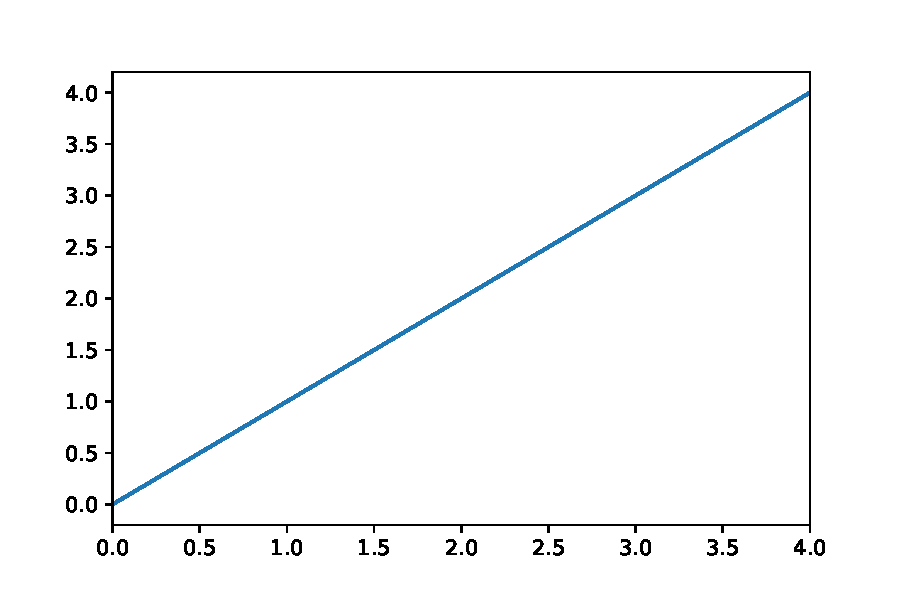
\includegraphics[width=0.7\textwidth]{fig/basicplot}
\pause

Saving the plot (e.g., to include in a report):
\begin{lstlisting}
ax = data.plot()
ax.figure.savefig('plot.pdf')  # or .png
\end{lstlisting}
\end{frame}

\begin{frame}[fragile]{Labeled data}
\begin{lstlisting}
In: data = pd.Series({'a': 0, 'b': 1})
\end{lstlisting}
The .index ...
\end{frame}

\begin{frame}[fragile]{A histogram}
\begin{lstlisting}
data.hist()
\end{lstlisting}
%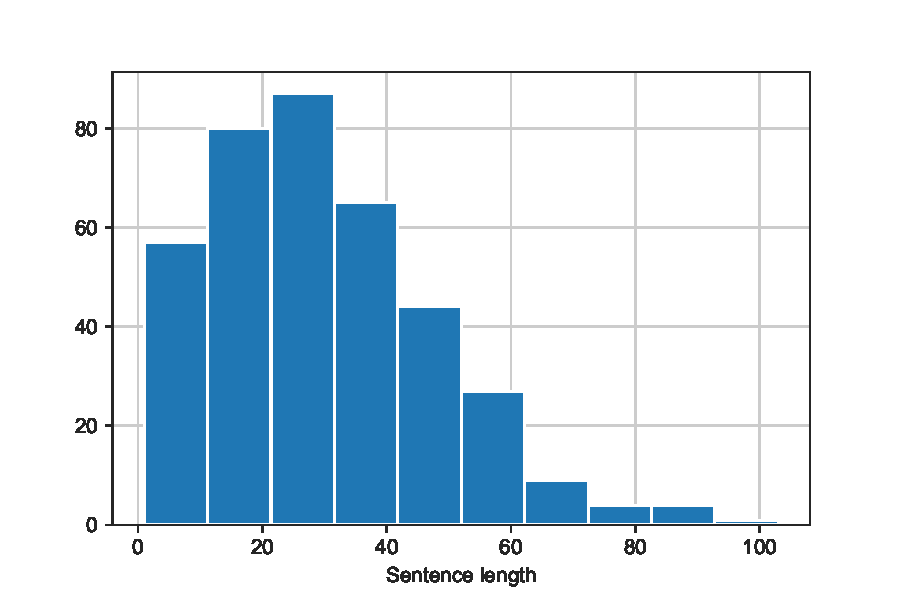
\includegraphics[width=0.7\textwidth]{fig/basichist}
\end{frame}

\begin{frame}[fragile]{Counting values}
% think of a new dataset
\begin{lstlisting}
data.value_counts()
\end{lstlisting}
\end{frame}

\begin{frame}[fragile]{Counting values: bar plot}
\begin{lstlisting}
counts = data.value_counts()
counts.plot.bar()
\end{lstlisting}
\end{frame}




\begin{frame}
Materials used for these slides:
\begin{itemize}
\item \url{https://www.cs.umd.edu/class/fall2018/cmsc320/}
    specifically lecture 11
    % https://www.cs.umd.edu/class/fall2018/cmsc320/lecs/cmsc320_f2018_lec11.pdf
\end{itemize}

\vspace{1em}
Documentation:
\begin{itemize}
    \item \url{http://pandas.pydata.org/pandas-docs/stable/}
\end{itemize}
\end{frame}

\end{document}
